\FloatBarrier
\section{Query-Modulated Models on Homogeneous, Sequential Benchmark\label{res:query-mod-sequential}}
To more explicitly compare performance to the non-query-modulated model, we narrow our focus to the combined data from all dimensions and examine the ratio of examples required to reach criterion between each query-modulation level and the baseline model, as we did for the control (sequential, heterogeneous dimensions) condition. Figure \ref{fig:results-query-mod-benchmark-examples-to-criterion-comparison} plots these ratios in a manner paralleling Figure \ref{fig:results-control-sequential-examples-to-criterion}. The top panels depict the ratio of examples required to reach criterion by the number of times a task was trained on. While all query-modulated models learn the earlier tasks introduced faster (points above the $y=1$ line), this advantage diminishes by the latter times the model was trained on earlier tasks. Surprisingly, models with query modulation at the first and second levels learn the last few tasks slightly slower (points above the $y=1$ line) than the baseline model. On the other hand, models with query modulation at the third and fourth levels show better relative performance, both retaining an advantage on the earlier tasks introduced until the final task, and showing approximately equal performance on the later tasks introduced. The bottom panels, comparing the ratio of examples to the criterion by the number of tasks the model is training on, depict a similar tale. All query-modulated models better earlier and the third and fourth levels remain better later. 

\begin{figure}[!htb]
% \vspace{-0.225in}
\centering
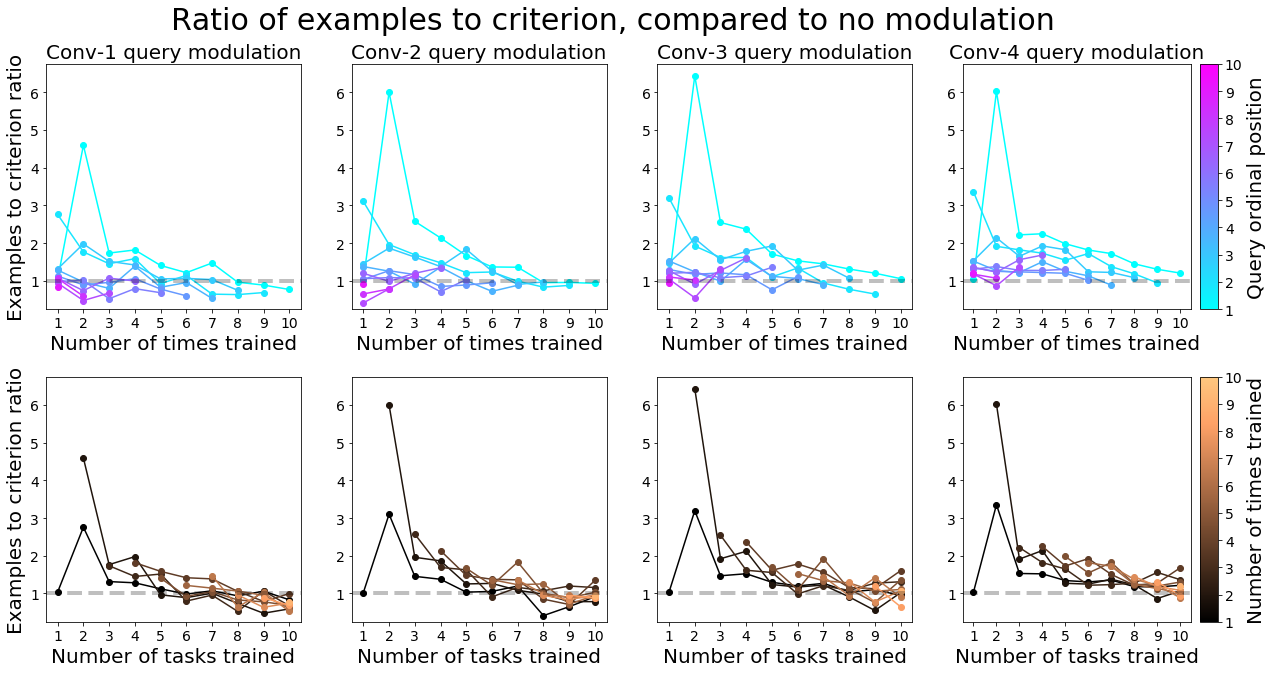
\includegraphics[width=\linewidth]{ch-results/figures/query_mod_benchmark/examples_to_criterion_comparison.png}
\caption[Ratio of examples to criterion.]{ {\bf Ratio of examples to criterion.} Comparing the ratio of examples to criterion, between each query-modulated model and the baseline model on the sequential, homogeneous dimension condition. We divide the number of examples the baseline model required by the number the query-modulated models needed, such that points above the $y=1$ line signify that the baseline model required longer training, and conversely, points below the line mark that the baseline model reached criterion faster. \textbf{Top:} Comparing by the number of times each task was trained on. \textbf{Bottom:} Comparing by the number of tasks the model trained on.}
\label{fig:results-query-mod-benchmark-examples-to-criterion-comparison}
% \vspace{-0.2in}
\end{figure}

Figure \ref{fig:results-query-mod-benchmark-first-task-accuracy-comparison} compares catastrophic forgetting patterns between the query-modulated models to the non-query-modulated baseline. As in Figure \ref{fig:results-control-sequential-first-episode-accuracy}, we take the difference between accuracies in the first epoch of a new episode, immediately after introducing a new task. The differences between the modulation levels in catastrophic forgetting are less drastic than in the examples to criterion: all query-modulation levels show less catastrophic forgetting in the first few times a task is trained, with narrowing advantage in the later repetitions on a given task. The same pattern emerges in the bottom panels, which compare based on the number of tasks trained.

\begin{figure}[!htb]
% \vspace{-0.225in}
\centering
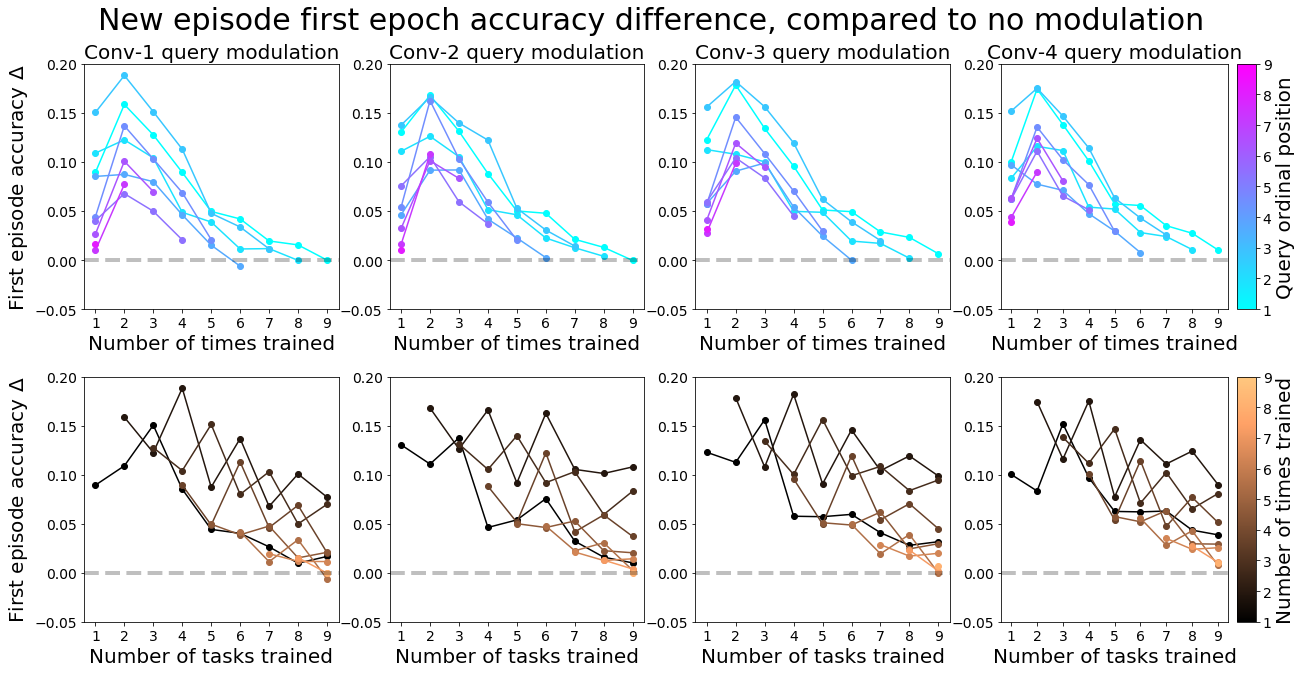
\includegraphics[width=\linewidth]{ch-results/figures/query_mod_benchmark/first_task_accuracy_comparison.png}
\caption[New episode first epoch accuracy difference.]{ {\bf New episode first epoch accuracy difference.} Comparing the difference in accuracies after training the first epoch of a new episode, between each query-modulated model and the baseline model on the sequential, homogeneous dimension condition. We subtract the accuracy the baseline model reached after the first episode from the accuracy the query-modulated models attained, such that points above the $y=0$ line signify that the baseline model showed worse catastrophic forgetting, and conversely, points below the line mark that the baseline model forgot less. \textbf{Top:} Comparing by the number of times each task was trained on. \textbf{Bottom:} Comparing by the number of tasks the model trained on. }
\label{fig:results-query-mod-benchmark-first-task-accuracy-comparison}
% \vspace{-0.2in}
\end{figure}

To statistically compare the performances of these different models, we considered the average on each of the fifty-five data points described above, of the average of the log of the number of examples to criterion, and performed a nonparametric sign test (see ch. 7 of \cite{Kvam2007}) on the differences between the models. We performed the sign test by subtracting the averages of one model from another, omitting any ties, and counting how many times one model did better than the other. Our null assumption is that the models perform approximately evenly, and therefore we would expect each model to perform better in about half of the comparisons. Therefore, we treat the comparisons as samples from a binomial distribution with $p = 0.5$ and the sample size set to the number of non-tie comparisons. We compute a two-sided $p$ value, which asks `if our null assumption was true, how often would we expect to see a result as extreme as the one we observed?' In other words, if the models perform equally well, the results of the comparisons should behave like coin flips from a fair coin; and if one model is better, it would appear more like a biased coin. This test is non-parametric, as it does not assume anything about the process generating the differences and only examines their signs. Table \ref{tab:log-examples-sign-test} depicts the result of a sign test comparing every pair of models to each other. The only two comparisons that fail to be statistically significant are between the baseline, non-query-modulated model and the first and second query-modulation level models. In every other case, the model modulating at a higher level performs better in the vast majority of the comparisons, suggesting that higher modulation levels confer some overall benefit to the number of examples required to reach criterion. 

\begin{table}[ht]
\centering
\caption{Log examples to criterion sign test}
\begin{threeparttable}
\begin{tabular}{@{}lllll@{}}
\toprule
 \thead[cl]{Modulation level}   & \thead[cl]{ 1 }                           & \thead[cl]{ 2 }                                & \thead[cl]{ 3 }                                & \thead[cl]{ 4 }                                \\
\midrule
 \thead[cl]{None}               & \makecell[cl]{ 27 $(n=55)$ \\ $p=1.0000$} & \makecell[cl]{ 34 $(n=55)$ \\ $p=0.1048$}      & \makecell[cl]{ 46 $(n=55)$ \\ $p=0.0000^{**}$} & \makecell[cl]{ 52 $(n=55)$ \\ $p=0.0000^{**}$} \\ \addlinespace[0.5em]
 \thead[cl]{ 1 }                &                                           & \makecell[cl]{ 41 $(n=55)$ \\ $p=0.0004^{**}$} & \makecell[cl]{ 51 $(n=55)$ \\ $p=0.0000^{**}$} & \makecell[cl]{ 54 $(n=55)$ \\ $p=0.0000^{**}$} \\ \addlinespace[0.5em]
 \thead[cl]{ 2 }                &                                           &                                                & \makecell[cl]{ 42 $(n=55)$ \\ $p=0.0001^{**}$} & \makecell[cl]{ 50 $(n=55)$ \\ $p=0.0000^{**}$} \\ \addlinespace[0.5em]
 \thead[cl]{ 3 }                &                                           &                                                &                                                & \makecell[cl]{ 42 $(n=54)$ \\ $p=0.0001^{**}$} \\
\bottomrule
\end{tabular}
\begin{tablenotes}
\item Sign test results on the differences between the log of the number of examples required to reach criterion, comparing the model in the row to the model in the column. For each sign test, we report the number of comparisons the model in the column did better on , the total sample size, and the sign test $p$ value. In all cases other than the first comparison (no modulation to first modulation level), the model in the column performed better (required fewer examples to criterion). $*: p < 0.05, **: p < 0.01$.
\end{tablenotes}
\end{threeparttable}
\label{tab:log-examples-sign-test}
\end{table}

We then devised a second way to perform this comparison, for which we could not find evidence in the literature, but we believe it increases the robustness of the procedure. In our alternative comparison, we also consider the standard errors of the means (SEMs) of the results from these models. We take an interval of one SEM around each of the results we are comparing, and if these intervals overlap, we consider this comparison as tied, rather than count it in the sign test. This correction process introduces ‘ties’ in every pair of comparisons we make, and reduces the effective sample size (as we omit ties), but it increases the robustness of our results, as we now require a difference to be beyond the margins of error to be considered as part of the sign test. Table \ref{tab:log-examples-sign-test-with-sem} shows the results after applying this correction. We see that all models besides the first query-modulated model outperform the baseline model and that the first query-modulated model it also outdone by the other query-modulated models.

\begin{table}[ht]
\centering
\caption{Log examples to criterion sign test with SEM}
\begin{threeparttable}
\begin{tabular}{@{}lllll@{}}
\toprule
 \thead[cl]{Modulation level}   & \thead[cl]{ 1 }                           & \thead[cl]{ 2 }                                & \thead[cl]{ 3 }                                & \thead[cl]{ 4 }                                \\ 
\midrule
 \thead[cl]{None}               & \makecell[cl]{ 12 $(n=17)$ \\ $p=0.1435$} & \makecell[cl]{ 15 $(n=17)$ \\ $p=0.0023^{**}$} & \makecell[cl]{ 23 $(n=24)$ \\ $p=0.0000^{**}$} & \makecell[cl]{ 31 $(n=31)$ \\ $p=0.0000^{**}$} \\ \addlinespace[0.5em]
 \thead[cl]{ 1 }                &                                           & \makecell[cl]{ 7 $(n=7)$ \\ $p=0.0156^{*}$}    & \makecell[cl]{ 8 $(n=8)$ \\ $p=0.0078^{**}$}   & \makecell[cl]{ 18 $(n=18)$ \\ $p=0.0000^{**}$} \\ \addlinespace[0.5em]
 \thead[cl]{ 2 }                &                                           &                                                & \makecell[cl]{ 2 $(n=2)$ \\ $p=0.5000$}        & \makecell[cl]{ 4 $(n=4)$ \\ $p=0.1250$}        \\ \addlinespace[0.5em]
 \thead[cl]{ 3 }                &                                           &                                                &                                                & \makecell[cl]{ 1 $(n=1)$ \\ $p=1.0000$}        \\
\bottomrule
\end{tabular}
\begin{tablenotes}
\item Similar sign test to Table \ref{tab:log-examples-sign-test}, but treating results where one standard error of the mean (SEM) intervals overlap as ties, rather than as differences counted for one of the models. The model in the column performed better than the model in the row in all cases. $*: p < 0.05, **: p < 0.01$.
\end{tablenotes}
\end{threeparttable}
\label{tab:log-examples-sign-test-with-sem}
\end{table}

We then repeated this comparison on the measure of catastrophic forgetting. We compared the forty-five first episode with new task test-set accuracies, which produced similar results to the training examples comparison reported above. Table \ref{tab:accuracy-sign-test} shows the raw results, without accounting for the SEMs. Save for the comparison between models modulating at the third and fourth level, every comparison is statistically significant, and all prefer the model modulating at a later processing level. Table \ref{tab:accuracy-sign-test-with-sem} (on the next page) depicts the results once we do account for the SEMs, as described above. All query-modulating models perform better than the baseline model, demonstrating once again that query-modulation confers benefits in catastrophic forgetting. Beyond that, the model modulating at the third convolution layer appears better than the one modulating at the first level, but barely so, as losing a single difference would push the p-value above 0.05. The only robust significant comparison is the model modulating at the fourth level outperforming the model modulating at the first one.

\begin{table}[ht]
\centering
\caption{New episode first epoch accuracy difference sign test}
\begin{threeparttable}
\begin{tabular}{@{}lllll@{}}
\toprule
\thead[cl]{Modulation level}   & \thead[cl]{ 1 }                                & \thead[cl]{ 2 }                                & \thead[cl]{ 3 }                                & \thead[cl]{ 4 }                                \\
\midrule
 \thead[cl]{None}               & \makecell[cl]{ 42 $(n=45)$ \\ $p=0.0000^{**}$} & \makecell[cl]{ 44 $(n=45)$ \\ $p=0.0000^{**}$} & \makecell[cl]{ 44 $(n=45)$ \\ $p=0.0000^{**}$} & \makecell[cl]{ 45 $(n=45)$ \\ $p=0.0000^{**}$} \\ \addlinespace[0.5em]
 \thead[cl]{ 1 }                &                                                & \makecell[cl]{ 33 $(n=45)$ \\ $p=0.0025^{**}$} & \makecell[cl]{ 41 $(n=45)$ \\ $p=0.0000^{**}$} & \makecell[cl]{ 37 $(n=45)$ \\ $p=0.0000^{**}$} \\ \addlinespace[0.5em]
 \thead[cl]{ 2 }                &                                                &                                                & \makecell[cl]{ 32 $(n=45)$ \\ $p=0.0066^{**}$} & \makecell[cl]{ 34 $(n=45)$ \\ $p=0.0008^{**}$} \\ \addlinespace[0.5em]
 \thead[cl]{ 3 }                &                                                &                                                &                                                & \makecell[cl]{ 29 $(n=45)$ \\ $p=0.0725$}      \\
\bottomrule
\end{tabular}
\begin{tablenotes}
\item Sign test results on the differences between the new episode, first epoch accuracies, comparing the model in the row to the model in the column. For each sign test, we report the number of comparisons the model in the column did better on , the total sample size, and the sign test $p$ value. The model in the column performed better than the model in the row in all cases (showed higher first epoch accuracy more often). $*: p < 0.05, **: p < 0.01$.
\end{tablenotes}
\end{threeparttable}
\label{tab:accuracy-sign-test}
\vspace{-0.1in}
\end{table}

\begin{table}[ht]
\vspace{-0.1in}
\centering
\caption{New episode first epoch accuracy difference sign test with SEM}
\begin{threeparttable}
\begin{tabular}{@{}lllll@{}}
\toprule
\thead[cl]{Modulation level}   & \thead[cl]{ 1 }                                & \thead[cl]{ 2 }                                & \thead[cl]{ 3 }                                & \thead[cl]{ 4 }                                \\
\midrule
\thead[cl]{None}               & \makecell[cl]{ 36 $(n=36)$ \\ $p=0.0000^{**}$} & \makecell[cl]{ 38 $(n=38)$ \\ $p=0.0000^{**}$} & \makecell[cl]{ 42 $(n=42)$ \\ $p=0.0000^{**}$} & \makecell[cl]{ 42 $(n=42)$ \\ $p=0.0000^{**}$} \\ \addlinespace[0.5em]
 \thead[cl]{ 1 }                &                                                & \makecell[cl]{ 3 $(n=4)$ \\ $p=0.6250$}        & \makecell[cl]{ 6 $(n=6)$ \\ $p=0.0312^{*}$}    & \makecell[cl]{ 12 $(n=12)$ \\ $p=0.0005^{**}$} \\ \addlinespace[0.5em]
 \thead[cl]{ 2 }                &                                                &                                                & \makecell[cl]{ 1 $(n=1)$ \\ $p=1.0000$}        & \makecell[cl]{ 6 $(n=7)$ \\ $p=0.1250$}        \\ \addlinespace[0.5em]
 \thead[cl]{ 3 }                &                                                &                                                &                                                & \makecell[cl]{ 2 $(n=3)$ \\ $p=1.0000$}        \\
\bottomrule
\end{tabular}
\begin{tablenotes}
\item Similar sign test to Table
\ref{tab:accuracy-sign-test}, but treating results where one standard error of the mean (SEM) intervals overlap as ties, rather than as differences counted for one of the models. The model in the column performed better than the model in the row in all cases. $*: p < 0.05, **: p < 0.01$.
\end{tablenotes}
\end{threeparttable}
\label{tab:accuracy-sign-test-with-sem}
\vspace{-0.1in}
\end{table}